\documentclass{../mathhomework}
\usepackage{enumitem}
\usepackage{graphicx}
\usepackage{float}
\usepackage{pdfpages}

% Assigment Info
\coursetitle{Linear Algebra}
\courseinstructor{Professor MacArthur}

\student{Carson Storm}

\assignmenttitle{Final Extra Credit}
\assignmentduedate{December 13, 2019}

\begin{document}
\maketitle

\pagebreak

The inner product is essential for many of the concepts used in Chapter 6, but so far we have only defined the inner product for
real number spaces, $\R^n$. In order to expand the notion of an inner product to other vector spaces we define a set of axioms
that a space's inner product must satisfy, so that we can define an inner product for other vector spaces. A inner product is an
operation that takes two vectors in the considered vectors space as operands and associated with them a real number. This inner
product can be used to define what a vector's length is, distances in the space as well as orthogonality. For example, be defining a
inner product for $\mathbb{P}^n$, we define what it means for two polynomials to be orthogonal. After defining the inner product we can
utilize concepts such as the Gram-Schmidt process, or solving Least-Squares problems in spaces that are not $\R^n$.

\pagebreak

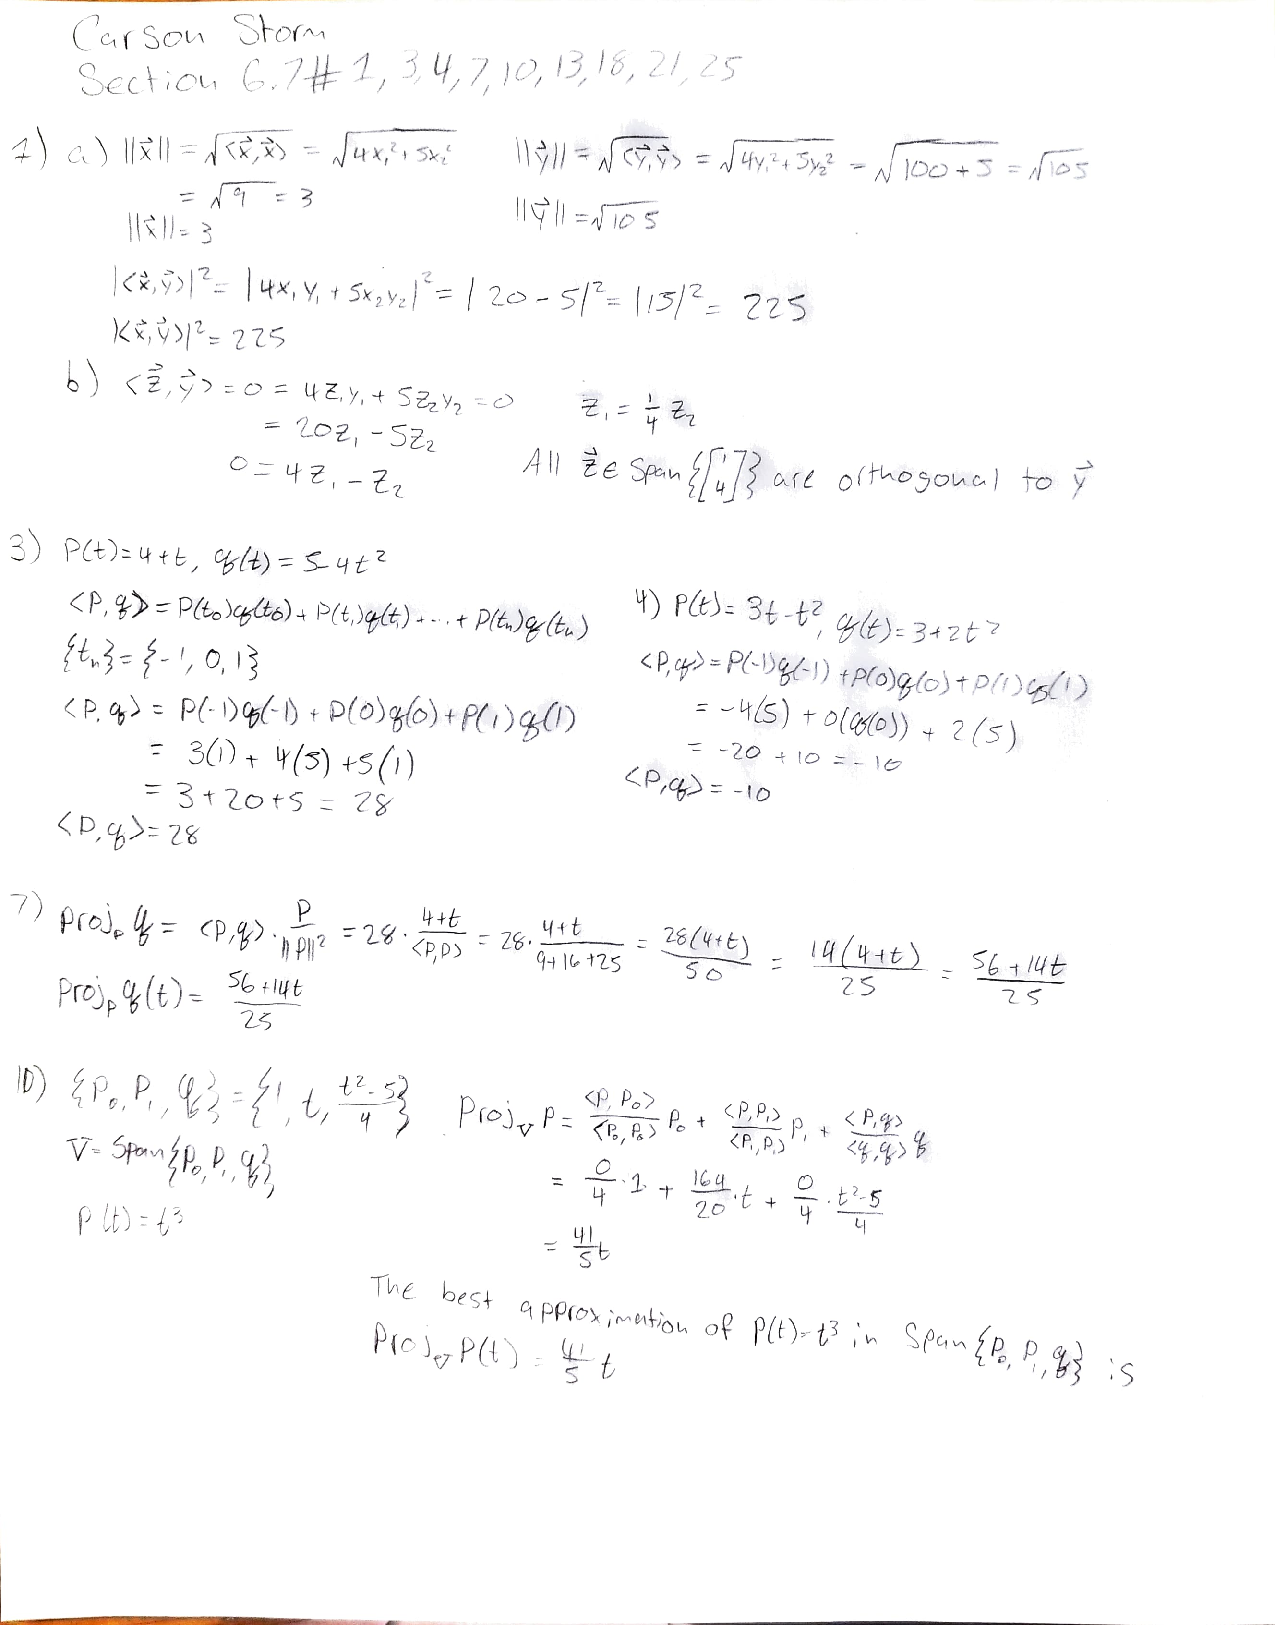
\includepdf[pages=-]{problems.pdf}

\end{document}